\section{Frattali} \label{sec:frattali}

Un frattale è un oggetto geometrico caratterizzato da due proprietà:
l'\emph{autosimilarità}, per cui la stessa struttura si ripete, identica o
statisticamente analoga, a scale di ingrandimento diverse, e una complessità di
dettaglio virtualmente infinita (figura~\ref{2_prop_fractals}). Un terzo tratto
riguarda il modo in cui i frattali vengono generati: non da una descrizione
statica, ma dalla \emph{ripetizione iterata di una regola semplice}
(figura~\ref{iteration_fractals}). Si distinguono tre grandi famiglie. I frattali
geometrici si costruiscono applicando ricorsivamente una trasformazione a una
figura di partenza, come il triangolo di Sierpiński, l'insieme di Cantor e la
curva di Koch (figura~\ref{Koch_fractals}). I frattali algebrici o
\emph{escape-time} si ottengono iterando una funzione sul piano complesso, come
l'insieme di Mandelbrot e gli insiemi di Julia. I frattali stocastici, infine,
introducono una componente casuale e descrivono molte forme naturali, come
alberi, fiumi, coste e nuvole~\cite{fractals_applications}.
\vspace{2mm}
\begin{figure}[H]
    \centering
    \begin{subfigure}[b]{0.4\textwidth}
        \centering
        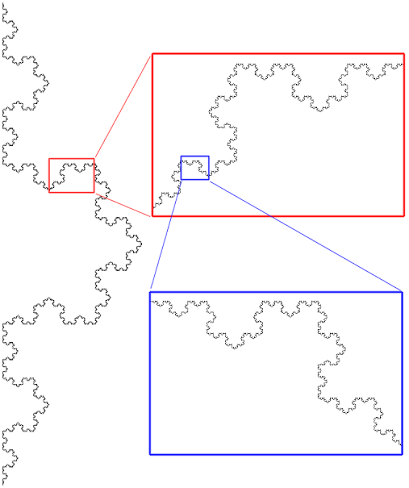
\includegraphics[width=6cm]{Immagini/images}
        \caption{Autosimilarità e complessità infinita.}
        \label{2_prop_fractals}
    \end{subfigure}
    \hspace{1cm}
    \begin{subfigure}[b]{0.4\textwidth}
        \centering
        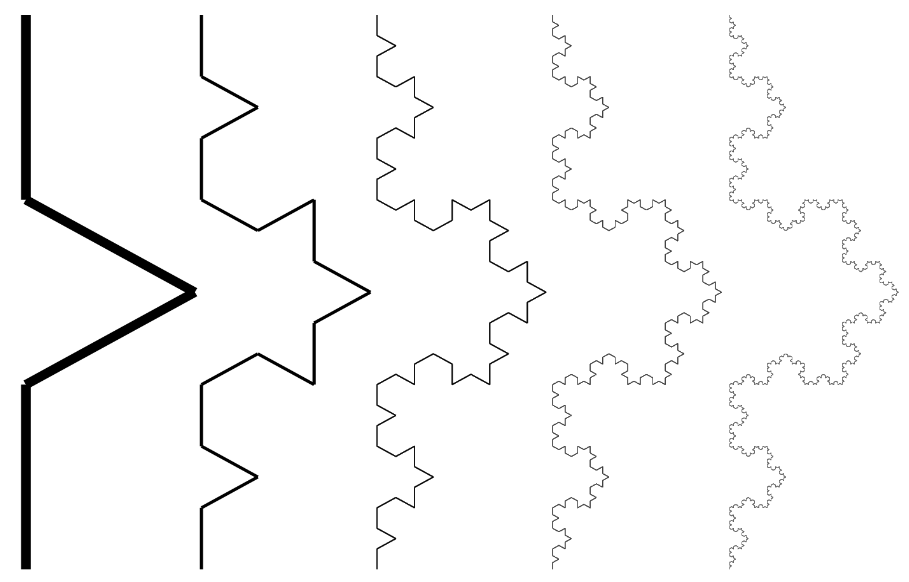
\includegraphics[width=\linewidth]{Immagini/koch_curve}
        \caption{Iterazioni nella figura.}
        \label{iteration_fractals}
    \end{subfigure}
    \caption{Curva di Koch: il fiocco di neve.}
    \label{Koch_fractals}
\end{figure}
\vspace{2mm}

\subsection{L'insieme di Mandelbrot}
\label{subsec:mandelbrot}

L'insieme di Mandelbrot è l'insieme dei numeri complessi $c$ per i quali la
successione
\[
\begin{cases}
    z_0 = 0 \\
    z_{n+1} = z_n^2 + c
\end{cases}
\]
rimane limitata~\cite{fractals_def}.

In accordo con la definizione di frattale, a ogni scala vi si ritrovano copie
ridotte dell'intero insieme, immerse in un intrico di filamenti
(figura~\ref{fig:autosimilarita}). L'autosimilarità è però solo approssimata: le
copie sono distorte e circondate da una filigrana ogni volta diversa. La
complessità, inoltre, non è distribuita in modo uniforme: le ampie regioni
interne ed esterne sono regolari, mentre i dettagli si concentrano sul
bordo~\cite{intro_fractals}.

\paragraph{Il calcolo del singolo pixel.}
Nell'implementazione il dominio è discretizzato in una griglia di $W \times H$
pixel. Al pixel di riga $i$ e colonna $j$, con $0 \leq i < H$ e $0 \leq j < W$,
corrisponde il punto del piano complesso
\[
c_{i,j} = \bigl(x_{\min} + (j + \tfrac{1}{2})\,dx\bigr) + \bigl(y_{\max} - (i + \tfrac{1}{2})\,dy\bigr)\,\mathrm{i},
\]
dove $dx = (x_{\max}-x_{\min})/W$ e $dy = (y_{\max}-y_{\min})/H$ sono i passi di
campionamento: le righe scandiscono la parte immaginaria, le colonne la parte
reale, e ogni pixel è rappresentato dal proprio centro.

Come anticipato nell'introduzione, il colore di ciascun pixel dipende soltanto
dal proprio $c$, e i pixel sono quindi indipendenti fra loro. Questa
indipendenza convive però con una dipendenza stretta all'interno del singolo
pixel. Fissato $c$, il calcolo dell'orbita\footnote{Per orbita di un punto $c$
si intende la successione $z_0, z_1, z_2, \dots$ associata a quel pixel. I
termini successione e orbita sono intercambiabili, con la sfumatura che il primo
enfatizza la lista ordinata di valori, mentre il secondo enfatizza il percorso
dinamico nel piano.} è intrinsecamente sequenziale, perché $z_{n+1}$ si calcola
solo una volta noto $z_n$. Il parallelismo del problema risiede quindi
\emph{fra} i pixel, non \emph{dentro} ciascuno di essi. Si noti infine la
duplice natura di $c$: distingue un pixel dall'altro ed è, allo stesso tempo, la
costante della successione $\{z_n\}$ associata a quel pixel.

\paragraph{Raggio di fuga e criterio di arresto.} \label{convergence}
Per la mappa $z \mapsto z^2 + c$ il valore $r = 2$ è un \emph{raggio di fuga}:
non appena $|z_n| > 2$, l'orbita diverge. Se infatti $|c| \leq 2$ e
$|z_n| > 2$, allora $|z_{n+1}| \geq |z_n|^2 - |c| > |z_n|$, e il modulo cresce a
ogni passo di una quantità che non diminuisce; se $|c| > 2$, già $|z_1| = |c|$
supera il raggio, e un argomento analogo mostra che l'orbita
diverge~\cite{fractals_def}. L'insieme di Mandelbrot $M$ è quindi il luogo dei
punti la cui orbita non supera mai il raggio di fuga:
\begin{equation}\label{equ:convergence}
    c \in M \iff |z_n| \leq 2 \quad \forall\, n \geq 0.
\end{equation}

Poiché per i punti di $M$ l'iterazione non terminerebbe mai, l'implementazione
usa due condizioni di arresto complementari.
\begin{enumerate}
    \item \emph{Fuga} (\emph{escape}): non appena $|z_n| > 2$, il punto è
    dichiarato esterno a $M$. Il numero di iterazioni eseguite è il \emph{tempo di
    fuga} (escape time) $n_{i,j}$. Dipende soltanto da $c$ ed è in generale tanto
    più piccolo quanto più $c$ è lontano dal bordo dell'insieme.
    \item \emph{Limite massimo di iterazioni} $N_{\max}$: se dopo $N_{\max}$ passi
    l'orbita non ha superato il raggio di fuga, il punto è considerato, in modo
    approssimato, interno a $M$, e il suo tempo di fuga vale $N_{\max}$.
\end{enumerate}

Il tempo di fuga varia quindi di ordini di grandezza da un pixel all'altro:
pochi passi per i punti lontani dall'insieme, centinaia o migliaia vicino al
bordo, $N_{\max}$ per i punti interni. È questa variabilità l'origine della
\textit{distribuzione non uniforme del lavoro} analizzata nelle sezioni
successive.

\paragraph{Struttura dell'insieme.}
% --- Figura: anatomia dell'insieme ---
\begin{figure}[H]
    \centering
    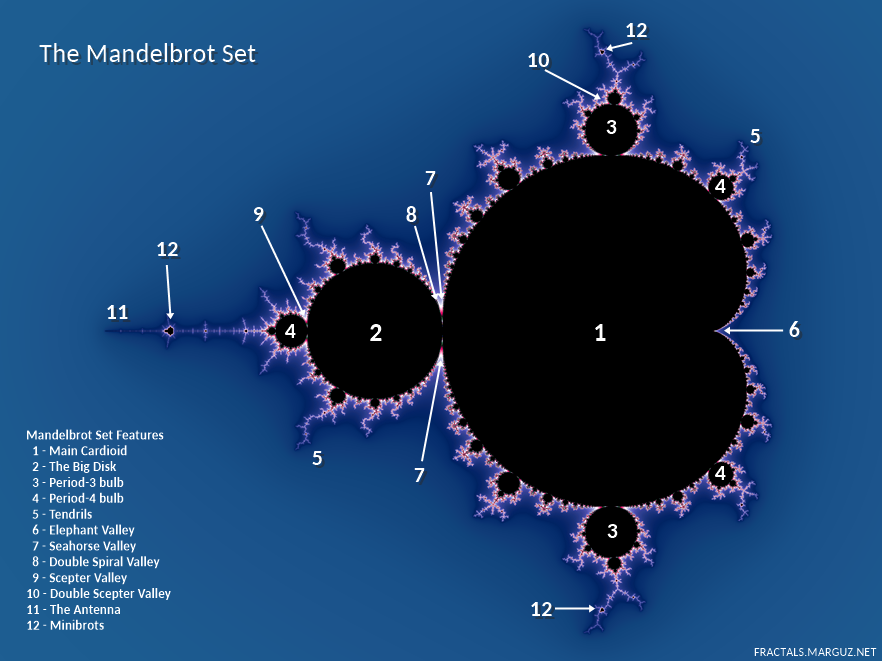
\includegraphics[width=0.85\linewidth]{Immagini/mandelbrot_elements}
    \caption{Anatomia dell'insieme di Mandelbrot~\cite{marguz_navigating}:
        (1)~cardioide principale; (2)~grande disco, il bulbo di periodo~2;
        (3)~bulbo di periodo~3; (4)~bulbo di periodo~4; (5)~filamenti; (6)~valle
        dell'elefante; (7)~valle del cavalluccio marino; (8)~valle della doppia
        spirale; (9)~valle dello scettro; (10)~valle del doppio scettro;
        (11)~antenna; (12)~minibrot.}
    \label{fig:mandelbrot_elements}
\end{figure}
L'insieme di Mandelbrot possiede un'anatomia riconoscibile
(figura~\ref{fig:mandelbrot_elements}). Il corpo principale è la
\emph{cardioide}, la regione in cui l'orbita di~$0$ è attratta da un punto fisso;
a essa è attaccato il \emph{bulbo di periodo~2}, il grande disco a sinistra, in
cui l'orbita è attratta invece da un ciclo di periodo~2. Intorno alla cardioide
si dispone un'infinità di \emph{bulbi primari}: per ogni punto $c$ di un bulbo di
periodo~$n$, l'orbita di~$0$ è attratta da un ciclo di periodo esattamente~$n$.
I bulbi secondari e terziari, attaccati ai primari, hanno periodo multiplo
di~$n$.

A ogni bulbo primario è associata un'\emph{antenna}, una struttura filiforme che
si prolunga verso l'esterno del bulbo e da cui partono più rami, detti
\emph{raggi} (\emph{spokes}). Il numero di raggi dell'antenna principale di un
bulbo è uguale al periodo del bulbo~\cite{bu_fracgeom}: l'antenna del bulbo di
periodo~3 ha tre raggi, quella del bulbo di periodo~5 ne ha cinque. I raggi
vanno distinti dai \emph{filamenti} (\emph{tendrils}), strutture diramate a ogni
scala che si estendono nella regione esterna e portano con sé infiniti
mini-Mandelbrot (\emph{minibrot}); i raggi, invece, compongono l'antenna di un
singolo bulbo.

Queste strutture determinano dove si concentra il lavoro: le righe che
attraversano la cardioide e il grande disco contengono molti punti interni,
ciascuno dei quali richiede $N_{\max}$ iterazioni, mentre bulbi, antenne e
filamenti portano pixel lenti a fuggire anche nella regione esterna.

\paragraph{Potenze superiori.}
La ricorrenza $z_{n+1} = z_n^2 + c$ si generalizza elevando $z_n$ a una potenza
intera $d \geq 2$:
\[
z_{n+1} = z_n^d + c.
\]
Gli insiemi che ne risultano conservano la struttura frattale di base, ma
cambiano simmetria: l'insieme per $d = 2$ è simmetrico rispetto all'asse reale,
quello per $d = 3$ ha simmetria di rotazione di ordine~2, e in generale l'insieme
di grado~$d$ presenta $d - 1$ bulbi principali equidistribuiti attorno
all'origine~\cite{maddmaths_mandelbulb}. Al crescere di~$d$ le strutture
diventano progressivamente più elaborate, e compaiono nuovi filamenti e bulbi
(figura~\ref{fig:mandelbrot_roots}).
\vspace{3mm}
\begin{figure}[H]
    \centering
    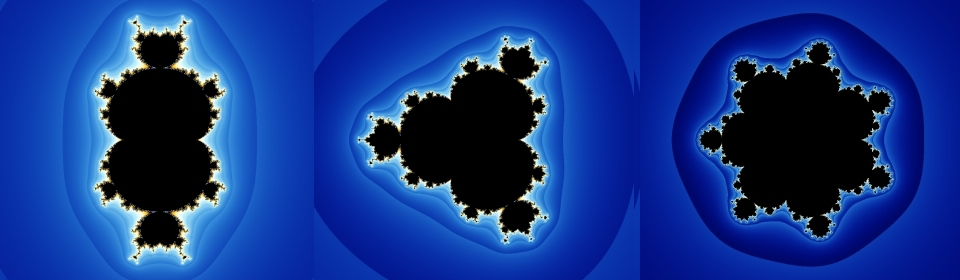
\includegraphics[width=0.85\linewidth]{Immagini/multiple_roots_mandelbrot}
    \caption{Insiemi di Mandelbrot generalizzati a potenze $d > 2$. Immagine
        tratta da~\cite{maddmaths_mandelbulb}.}
    \label{fig:mandelbrot_roots}
\end{figure}

\paragraph{La colorazione escape-time.} \label{work_load_visualization}
La colorazione \emph{escape-time} assegna a ciascun pixel esterno un colore in
funzione del proprio tempo di fuga e lascia in nero i pixel classificati come
interni. Nelle figure di questo lavoro la scala è logaritmica: i punti che
fuggono in pochi passi, lontani dall'insieme, sono blu scuro, e le bande si
schiariscono verso il bianco e l'ambra avvicinandosi al bordo
(figura~\ref{fig:autosimilarita}). Le fughe più lente, oltre circa $400$
iterazioni, tornano però verso tonalità scure. La forma nera è quindi solo
un'approssimazione di $M$: contiene anche i punti che fuggirebbero dopo più di
$N_{\max}$ iterazioni, e la sua accuratezza cresce con $N_{\max}$ e con la
risoluzione, al prezzo di un costo di calcolo maggiore. L'alone colorato attorno
all'insieme non aggiunge invece informazione sulla forma, perché dipende soltanto
dalla palette scelta.

\begin{figure}[H]
    \centering
    \begin{subfigure}[b]{0.4\textwidth}
        \centering
        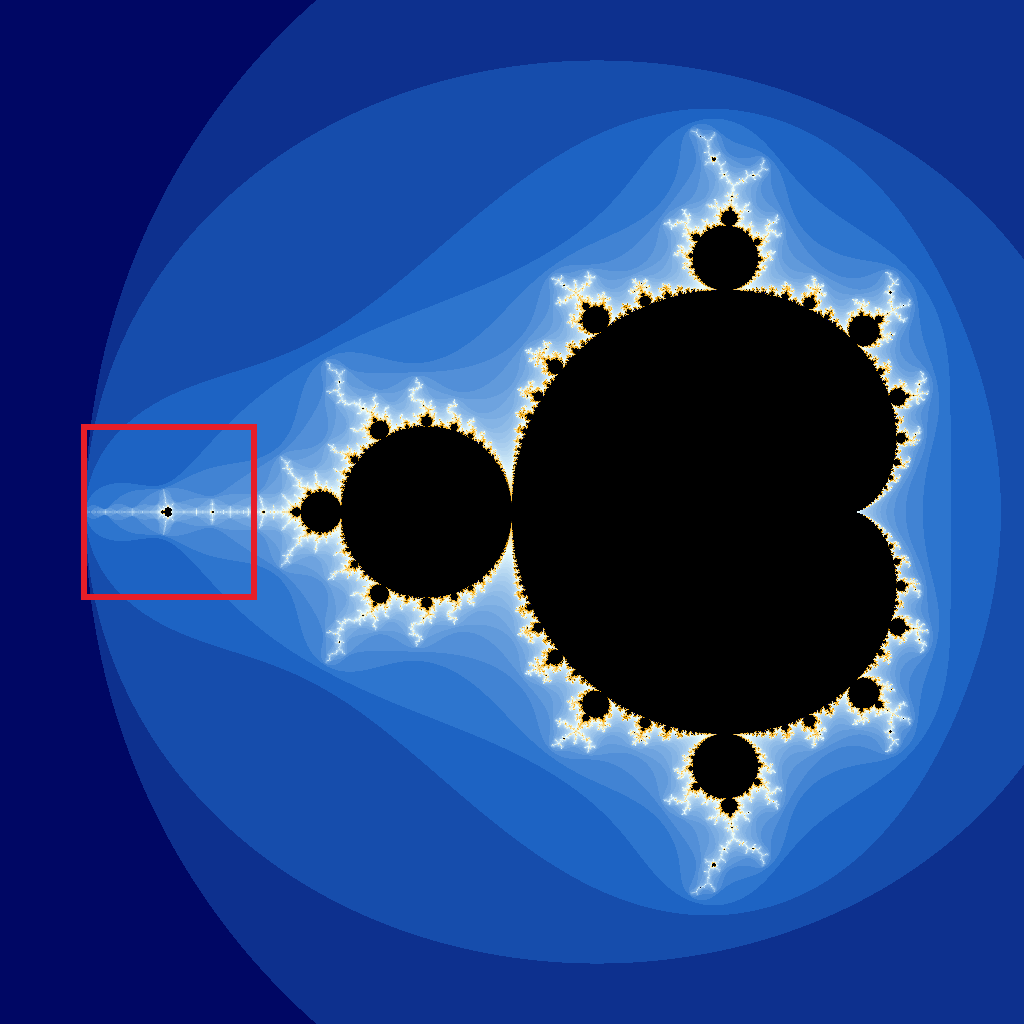
\includegraphics[width=\linewidth]{Immagini/frattali/zoom1_insieme}
        \caption{L'insieme completo}
        \label{fig:zoom_insieme}
    \end{subfigure}
    \hspace{0.5cm}
    \begin{subfigure}[b]{0.4\textwidth}
        \centering
        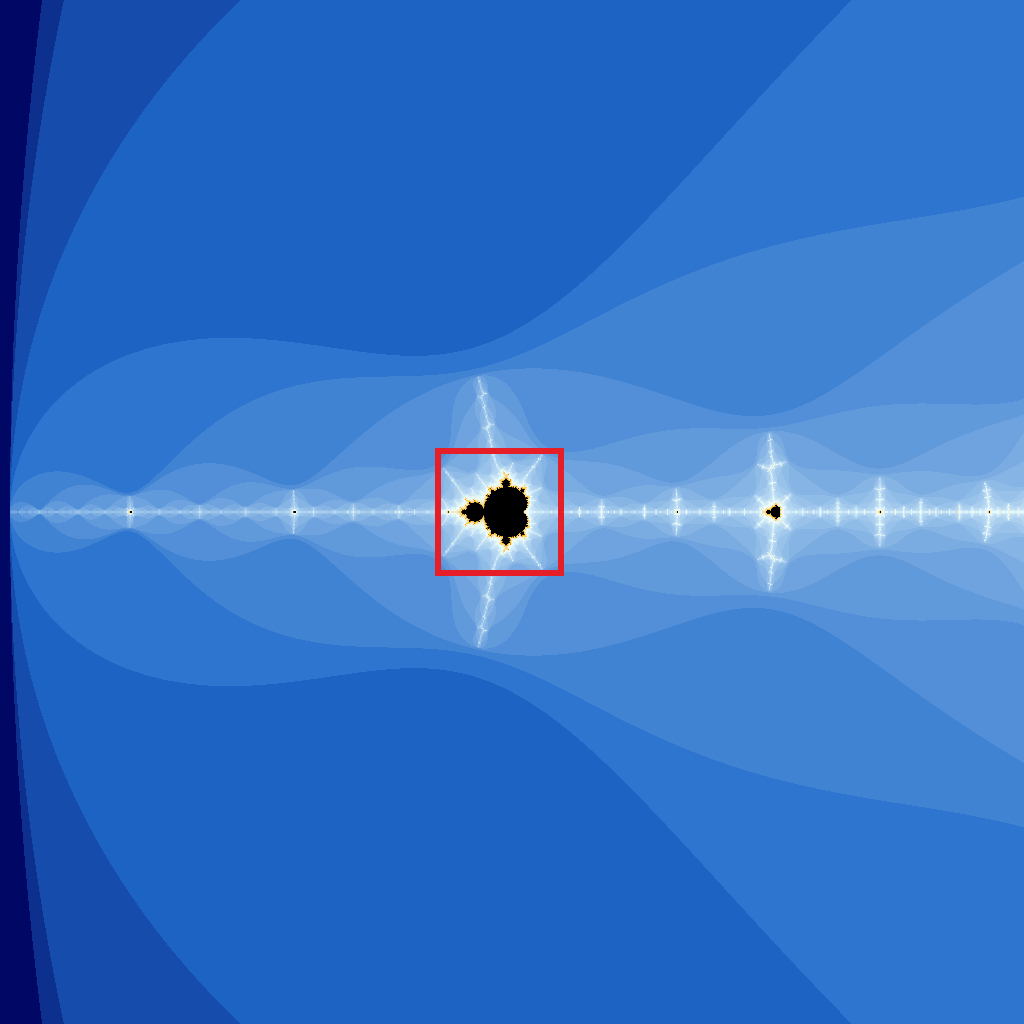
\includegraphics[width=\linewidth]{Immagini/frattali/zoom2_antenna}
        \caption{Ingrandimento $6\times$}
        \label{fig:zoom_antenna}
    \end{subfigure}

    \vspace{4mm}

    \begin{subfigure}[b]{0.4\textwidth}
        \centering
        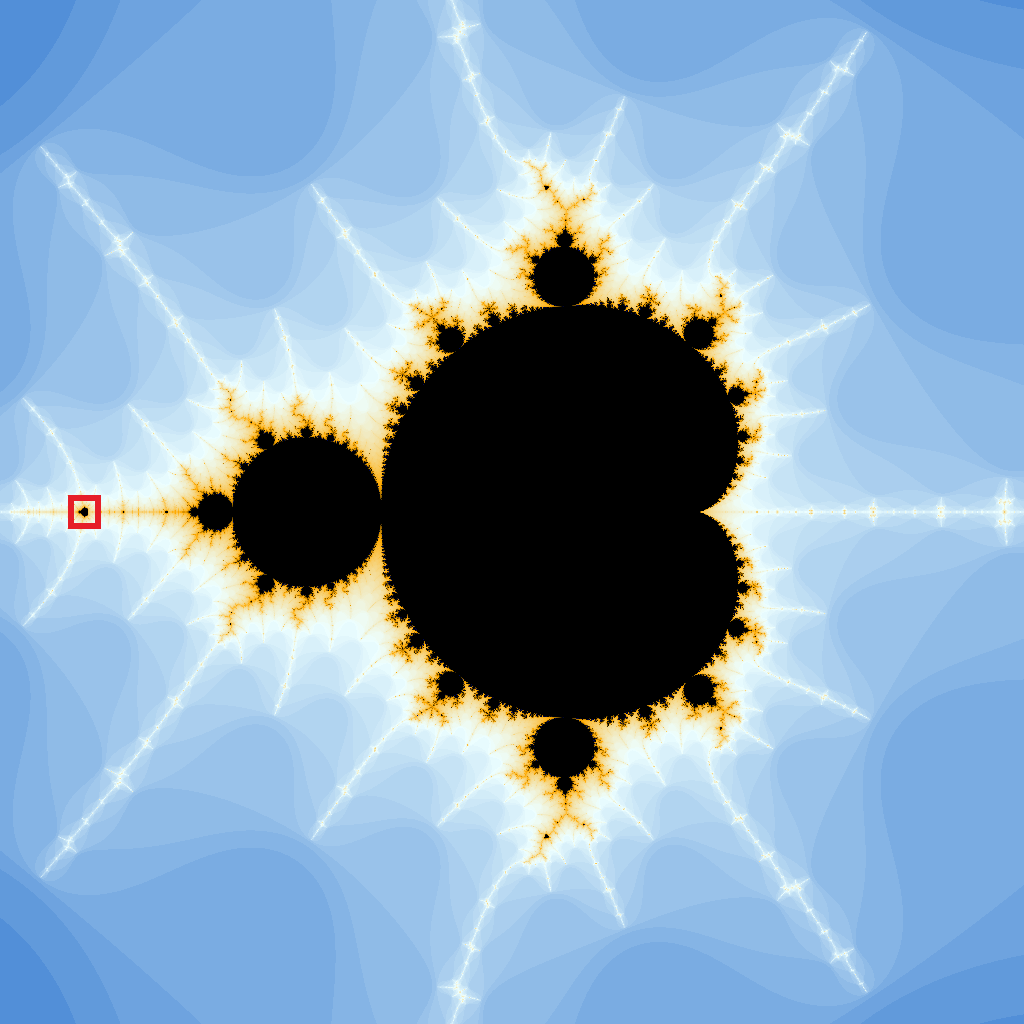
\includegraphics[width=\linewidth]{Immagini/frattali/zoom3_isola}
        \caption{Ingrandimento $50\times$}
        \label{fig:zoom_isola}
    \end{subfigure}
    \hspace{0.5cm}
    \begin{subfigure}[b]{0.4\textwidth}
        \centering
        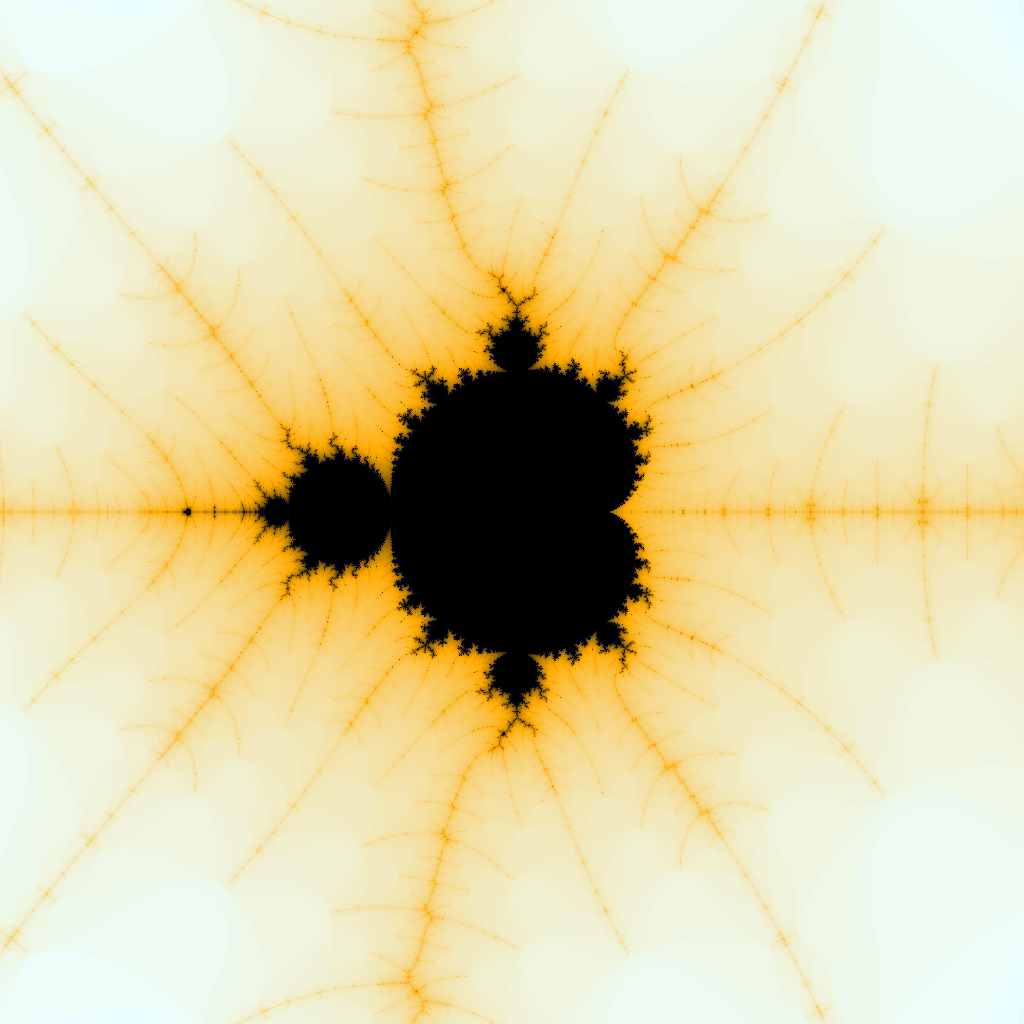
\includegraphics[width=\linewidth]{Immagini/frattali/zoom4_sottoisola}
        \caption{Ingrandimento $1875\times$}
        \label{fig:zoom_sottoisola}
    \end{subfigure}
    \caption{Autosimilarità dell'insieme di Mandelbrot. Quattro finestre annidate
        l'una dentro l'altra, tutte calcolate dal codice seriale di questo lavoro, a
        risoluzione $1024 \times 1024$ e con $N_{\max}=1000$ \emph{fisso}: fra un
        pannello e il successivo cambia unicamente la porzione di piano complesso
        campionata, indicata dal riquadro rosso. (a) L'insieme completo,
        $[-2{,}25;\,0{,}75] \times [-1{,}5;\,1{,}5]$. (b) La coda dell'antenna,
        centro $c=-1{,}7548776$, lato $0{,}5$: sull'asse reale si allineano alcuni
        nuclei scuri. (c) Uno di essi, centro $c=-1{,}7608776$, lato $0{,}06$:
        ricompaiono la cardioide, il bulbo di periodo~2 e la corona di bulbi minori
        dell'insieme completo. (d) Il nucleo evidenziato sull'antenna della copia
        precedente, centro $c=-1{,}7859250$, lato $1{,}6 \cdot 10^{-3}$: la stessa
        struttura si ripresenta una terza volta, e si può continuare
        indefinitamente. Il riquadro in (c) è molto piccolo, perché la copia di (d)
        è circa $40$ volte più piccola di quella che la contiene: è questa
        gerarchia di scale a produrre la complessità di dettaglio virtualmente
        infinita. I quattro pannelli condividono la stessa scala di colore, per cui
        una data tinta corrisponde sempre allo stesso numero di iterazioni: lo
        sfondo che si scalda progressivamente misura la crescita del tempo di fuga
        minimo con la profondità dell'ingrandimento, che passa da $1$ iterazione in
        (a) a $25$ in (d).}
    \label{fig:autosimilarita}
\end{figure}
\vspace{2mm}

\subsection{Pseudocodice} \label{pseudo}
\vspace{3mm}
\begin{pseudocode}
\label{alg:escape_time}
\begin{algorithmic}[1]
\For{each pixel ($P_x, P_y$) on the screen}
    \State $x_0 \gets \text{scaled } x \text{ coordinate of pixel}$
    \State $y_0 \gets \text{scaled } y \text{ coordinate of pixel}$
    \State $x \gets 0$,\quad $y \gets 0$,\quad $x_{\mathrm{sq}} \gets 0$,\quad $y_{\mathrm{sq}} \gets 0$,\quad $iteration \gets 0$
    \While{$x_{\mathrm{sq}} + y_{\mathrm{sq}} \leq 4$ \textbf{ and } $iteration < \mathit{max\_iteration}$}
        \State $y \gets 2xy + y_0$
        \State $x \gets x_{\mathrm{sq}} - y_{\mathrm{sq}} + x_0$
        \State $x_{\mathrm{sq}} \gets x^2$,\quad $y_{\mathrm{sq}} \gets y^2$
        \State $iteration \gets iteration + 1$
    \EndWhile
    \State $\mathit{plot}(P_x,\, P_y,\; \mathit{palette}[iteration])$
\EndFor
\end{algorithmic}
\end{pseudocode}
\noindent dove $z = x + \mathrm{i}\,y$, $c = x_0 + \mathrm{i}\,y_0$ e
$\mathit{max\_iteration} = N_{\max}$. L'algoritmo~\ref{alg:escape_time} traduce la
definizione in istruzioni eseguibili e adotta tre accorgimenti.

\begin{itemize}
    \item \textbf{Test di fuga senza radice quadrata.} Il
    criterio~\eqref{equ:convergence} richiederebbe il modulo
    $|z_n| = \sqrt{x^2 + y^2}$, e la radice quadrata in virgola mobile è
    sensibilmente più costosa di moltiplicazioni e addizioni. Poiché entrambi i
    membri sono non negativi, la condizione si eleva al quadrato senza cambiarne il
    significato, e la fuga diventa
    \[
    x^2 + y^2 > 4.
    \]

    \item \textbf{Scomposizione in parte reale e immaginaria.} L'hardware non
    dispone di un tipo complesso nativo e opera su registri in virgola mobile.
    Sviluppando
    \[
    z^2 = (x + \mathrm{i}\,y)^2 = x^2 - y^2 + 2\,\mathrm{i}\,xy,
    \]
    la ricorrenza diventa un sistema di due equazioni reali accoppiate:
    \[
    \begin{cases}
        x_{n+1} = x_n^2 - y_n^2 + x_0\\
        y_{n+1} = 2\,x_n y_n + y_0
    \end{cases}
    \]

    \item \textbf{Riuso dei quadrati.} I valori $x^2$ e $y^2$ servono sia
    all'aggiornamento di $x$ sia al test di fuga: memorizzandoli si calcolano una
    sola volta, e le moltiplicazioni per iterazione scendono da $6$ a $4$. Il costo
    per iterazione che ne risulta, $\varphi = 8$ FLOP, è ricavato nella
    sezione~\ref{sec:lavoro}.
\end{itemize}

Esistono inoltre ottimizzazioni strutturali che sfruttano proprietà
geometriche e di simmetria dell'insieme --- il pre-screening analitico
della cardioide e lo sfruttamento della simmetria assiale ---
la cui trattazione è rimandata alla sezione~\ref{sec:ottimizzazioni},
dopo aver introdotto il contesto implementativo necessario.
